\documentclass[reqno]{standalone}
% check https://latexdraw.com/automata-diagrams-in-latex/
\usepackage{tikz}
\usetikzlibrary{automata}
\usetikzlibrary{positioning}  %                 ...positioning nodes
\usetikzlibrary{arrows}       %                 ...customizing arrows
\tikzset{node distance=4.5cm, % Minimum distance between two nodes. Change if necessary.
         every state/.style={ % Sets the properties for each state
           semithick,
           draw = red, fill = red!30},
         initial text={},     % No label on start arrow
         double distance=4pt, % Adjust appearance of accept states
         every edge/.style={  % Sets the properties for each transition
         draw,
           ->,>=stealth',     % Makes edges directed with bold arrowheads
           auto,
           semithick}}

\begin{document}

\begin{figure}[htb]
\centering
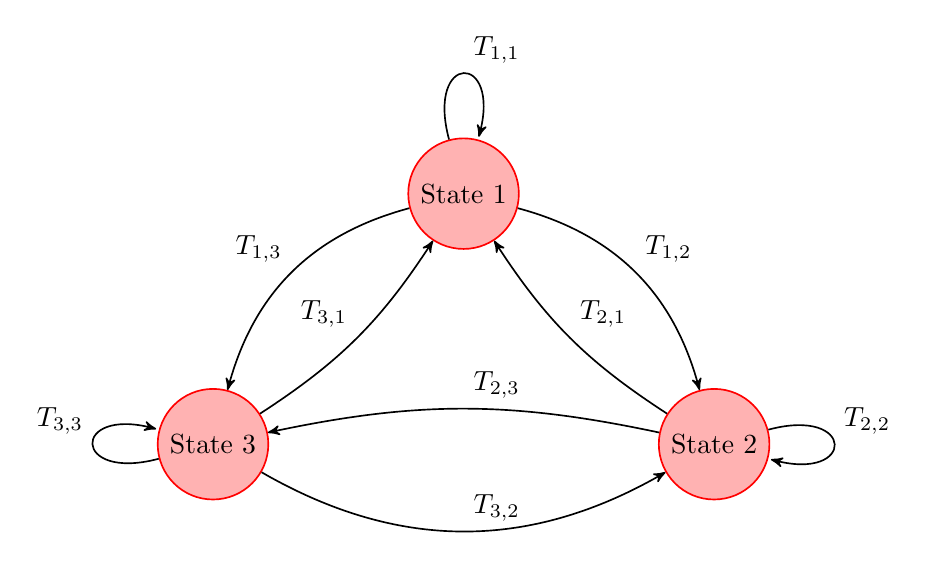
\begin{tikzpicture}
\node[state] (s1) {State 1};
\node[state, below right of=s1] (s2) {State 2};
\node[state, below left of=s1] (s3) {State 3};

\draw (s1) edge[loop above] node[above right] {$T_{1,1}$} (s1);
\draw (s1) edge[bend left] node[above right] {$T_{1,2}$} (s2);
\draw (s1) edge[bend right] node[above left] {$T_{1,3}$} (s3);

\draw (s2) edge[bend left=12] node[above right] {$T_{2,1}$} (s1);
\draw (s2) edge[loop right] node[above right] {$T_{2,2}$} (s2);
\draw (s2) edge[bend right=12] node[above right] {$T_{2,3}$} (s3);

\draw (s3) edge[bend right=12] node[above left] {$T_{3,1}$}  (s1);
\draw (s3) edge[bend right] node[above right] {$T_{3,2}$} (s2);
\draw (s3) edge[loop left] node[above left] {$T_{3,3}$} (s3);

\end{tikzpicture}
\end{figure}
\end{document}
